\documentclass[xcolor=dvipsnames, aspectratio=169]{beamer}
\usepackage[ngerman]{babel}
\usepackage{amsmath}
\usepackage{amssymb}
\usepackage{amsfonts}
\usepackage{mathpazo}
\usepackage{enumerate}
\usepackage{tikz}
\usepackage[version=4,arrows=pgf-filled]{mhchem}
\usepackage{mathdots}
\usepackage{multirow}
\usepackage{booktabs}
\usepackage{tabularx}
\usetikzlibrary{matrix,backgrounds,patterns,arrows,decorations.markings,shapes}
\usepackage{caption}

\usetheme[titleformat title=regular,titleformat frame=regular,titleformat section=allcaps,numbering=fraction]{metropolis} 
%\setsansfont[BoldFont={Fira Sans SemiBold}]{Fira Sans Book}
%\setmonofont[Scale=1.1]{Ubuntu Mono}

\mhchemoptions{mathfontcommand=\mathsf}

\author[Felix Kußmaul]{\large Felix Kußmaul}
\title[NAA]{\Large Die Neutronenaktivierungsanalyse}
\subtitle{Einführung und Anwendungen in der Archäologie}
\institute[UzK]{Seminar zu naturwissenschaftlichen Untersuchungsmethoden\\ von Fundkeramik und ihrer archäologischen Interpretation\\[.5em] Universität zu Köln}
\date[23.\ Juli 2016]{23.\ Juli 2016}

\newcommand{\red}[1]{\textcolor{red}{#1}}
\newcommand{\orange}[1]{\textcolor{orange}{#1}}
\newcommand{\green}[1]{\textcolor{markgreen}{#1}}
\newcommand{\textgreen}[1]{\textcolor{textgreen}{#1}}
\newcommand{\blue}[1]{\textcolor{textblue}{#1}}
\newcommand{\gray}[1]{\textcolor{gray}{#1}}

\newcolumntype{R}{>{\centering\raggedleft\arraybackslash}X}
\newcolumntype{L}{>{\centering\raggedright\arraybackslash}X}
\newcolumntype{C}{>{\centering\arraybackslash}X}

\usepackage[firstinits=true,style=archaeologie,width=2cm,edby,backend=biber]{biblatex}
\addbibresource{naa.bib}
\renewcommand*{\bibfont}{\small}

\setbeamercovered{invisible}

\newcommand{\textsb}[1]{{\fontfamily{cmss}\fontseries{sbc}\fontshape{n}\selectfont #1}}

\setbeamertemplate{footline}
{
\hbox{%
  \begin{beamercolorbox}[wd=.28\paperwidth,ht=2.7ex,dp=1.2ex,center]{author in head/foot}%
    \usebeamerfont{author in head/foot}\insertshortauthor\ (\insertshortinstitute)
  \end{beamercolorbox}%
  \begin{beamercolorbox}[wd=.44\paperwidth,ht=2.7ex,dp=1.2ex,center]{author in head/foot}%
    \usebeamerfont{title in head/foot}\insertshorttitle:\ \textbf{\insertsection}
  \end{beamercolorbox}%
  \begin{beamercolorbox}[wd=.28\paperwidth,ht=2.7ex,dp=1.2ex,center]{author in head/foot}%
    \usebeamerfont{date in head/foot}\insertshortdate\hfill\insertframenumber/\inserttotalframenumber\strut
  \end{beamercolorbox}}
  \vskip0pt%
}

\tikzset{
  invisible/.style={opacity=0},
  visible on/.style={alt={#1{}{invisible}}},
  alt/.code args={<#1>#2#3}{%
    \alt<#1>{\pgfkeysalso{#2}}{\pgfkeysalso{#3}} % \pgfkeysalso doesn't change the path
  },
}

\newcommand{\printSectionYes}{\AtBeginSubsection[]
{
 \begin{frame}{Agenda}
 \tableofcontents[sectionstyle=show/shaded,
 					subsectionstyle=show/shaded/hide]
 \end{frame}
}}

\tikzset{onslide/.code args={<#1>#2}{%
  \only<#1>{\pgfkeysalso{#2}}%
}}

\setbeamertemplate{section in toc shaded}[default][50]

\setbeamertemplate{subsection in toc shaded}[default][50]

\makeatletter
\patchcmd{\beamer@sectionintoc}{\vskip1.5em}{\vskip0.5em}{}{}
\makeatother

\makeatletter
\newcommand\footnoteref[1]{\protected@xdef\@thefnmark{\ref{#1}}\@footnotemark}
\makeatother

\setbeamertemplate{bibliography item}{%
  \ifboolexpr{ test {\ifentrytype{book}} or test {\ifentrytype{mvbook}}
    or test {\ifentrytype{collection}} or test {\ifentrytype{mvcollection}}
    or test {\ifentrytype{reference}} or test {\ifentrytype{mvreference}} }
    {\setbeamertemplate{bibliography item}[book]}
    {\ifentrytype{online}
       {\setbeamertemplate{bibliography item}[online]}
       {\setbeamertemplate{bibliography item}[article]}}%
  \usebeamertemplate{bibliography item}}
  
\defbibenvironment{bibliography}
  {\list{}
     {\settowidth{\labelwidth}{\usebeamertemplate{bibliography item}}%
      \setlength{\leftmargin}{\labelwidth}%
      \setlength{\labelsep}{\biblabelsep}%
      \addtolength{\leftmargin}{\labelsep}%
      \setlength{\itemsep}{\bibitemsep}%
      \setlength{\parsep}{\bibparsep}}}
  {\endlist}
  {\item}
\pgfdeclareimage[width=\columnwidth]{snucleus}{snucleus.eps}
\definecolor{morange}{HTML}{FF8200}
 
\begin{document}

\maketitle

\begin{frame}[<+->]{Before we start \dots}
\begin{itemize}
\item Zu langsam/schnell/undeutlich? \textbf{Bitte meckern!}
\item Fragen \alert{jederzeit} willkommen
\item Du sollst keine anderen Editoren neben \texttt{vim} haben
\item \LaTeX\ $\gg$ MS PowerPoint
\end{itemize}
\end{frame}

\begin{frame}{Agenda}
       \tableofcontents[ 
  		subsectionstyle=show, 
   	 	sectionstyle=show, 
   	 ] 
\end{frame}

\section{Einordnung}\printSectionYes

\begin{frame}{Sinn und Zweck}
\begin{quote}
``NAA is a sensitive analytical technique useful for performing both qualitative and quantitative \alert{multi-element analysis} of major, minor, and trace elements in samples from almost every conceivable field of scientific or technical interest.''
\end{quote}
\vspace*{-2em}
\begin{flushright}
-- Dr.\ Michael Glascock, MURR
\end{flushright}
\end{frame}

\begin{frame}{\dots\ in der Archäologie}
Wir Archäologen nutzen NAA seit Jahrzehnten erfolgreich für
\begin{itemize}
\item die Bestimmung der \textbf{Herkunft} eines Objektes
\item die Überprüfung der \textbf{Echtheit} eines fragwürdigen Gegenstandes
\item Studien zur \textbf{Herstellung} und \textbf{Nutzung} von Artefakten
\end{itemize}
\end{frame}

\begin{frame}{Herkunftsbestimmung}
Wir treffen folgende wichtige Annahmen:
\begin{enumerate}[(i)]
\item Kein Handel mit Rohton
\item Bei hoher Präzision gilt ein Elementmuster als \textbf{charakteristisch} für einen Ort
\item Gefäße mit gleichem Elementmuster stammen vom selben Ort
\item Das Muster veränderte sich nicht über die Zeit
\end{enumerate}
\end{frame}

\begin{frame}{Herkunftsbestimmung}
\begin{center}\Large
\begin{tabularx}{.9\columnwidth}{rlCrl}
\multirow{2}{*}{\parbox[c]{4.5em}{
\includegraphics[scale=.6]{pot}}}&&&&\multirow{2}{*}{\parbox[c]{4.5em}{
\includegraphics[scale=.6]{pot}}}\\
&\vphantom{$\overset{?}{=}$}\only<2-3>{Herkunft$_A$&$\overset{?}{=}$&Herkunft$_B$}&\\
&\onslide<3>{Muster$_A$&$=$&Muster$_B$}&\\
\end{tabularx}
\end{center}
\end{frame}
\begin{frame}{Herkunftsbestimmung}
\begin{center}\Large
\begin{tabularx}{.9\columnwidth}{rlCrl}
\multirow{2}{*}{\parbox[c]{4.5em}{
\includegraphics[scale=.6]{pot}}}&&&&\multirow{2}{*}{\parbox[c]{4.5em}{
\includegraphics[scale=.6]{pot}}}\\
&\color{morange}\vphantom{$\overset{?}{=}$}Herkunft$_A$&\color{morange}\vspace*{-1em}$=$&\color{morange}Herkunft$_B$&\\
&Muster$_A$&$=$&Muster$_B$&\\
\end{tabularx}
\end{center}
\end{frame}

\begin{frame}{Herkunftsbestimmung}
\textbf{Bekannte Herausforderungen:}
\begin{itemize}[<+->]
\item Nur selten wurde Rohton direkt verwendet.

\textit{Meist wurde er vor dem Töpfern gesäubert oder mit anderem Ton vermischt.}
\item Variation bei der Aufbereitung führt zur Veränderung der Zusammensetzung.

\textit{Die Konzentrationswerte müssen relativ zueinander betrachtet werden.}
\item Veränderungen durch Brand und Bodenlagerung für bestimmte Elemente.

\textit{Die betroffenen Elemente werden bei der Messung nicht berücksichtigt.}
\item Messungenauigkeiten oder -fehler.
\end{itemize}
\end{frame}

\begin{frame}{Herkunftsbestimmung}
\textbf{Problem mit Streuungen}

Gewisse Streuungen (5--10\,\%) sind normal für Proben mit homogener Masse.

Zur Einteilung in Gruppen von Proben wollen wir nicht mehr als diesen Toleranzbereich zulassen, da sonst das zu \glqq diffuse\grqq\ Gesamtmuster eine Unterscheidung verschiedener Herkünfte stark erschwert.
\end{frame}

\begin{frame}{Zuordnung: Muster $\mapsto$ Werkstatt, VLLT STREICHEN?!}
\begin{itemize}
\item Schwerster Schritt.
\item Notwendig: Finden von Referenzmaterial \textit{für jede Produktionsserie}.

Dafür gut geeignet sind \alert{Fehlbrände} aus Abfallhaufen.\medskip\pause

Alternativ: Logische Schlüsse anhand von \alert{Verteilungen}:

Lokale Produktion genau dann, wenn chemisches Muster dort in großen Stückzahlen gefunden wurde (nicht nur Keramik)
\end{itemize}
\end{frame}

\section{Methode}

\subsection{Probenherstellung}

\begin{frame}{Schritt 1: Probenentnahme}
\begin{minipage}{0.56\textwidth}\flushleft
\textbf{Entnahme der Probe vom Fundstück:}\smallskip

\begin{itemize}
\item mit Schaber o.\ Spitzbohrer

$\Rightarrow$ chemisch rein, z.\,B.\ synth.\ Saphir
\item z.\,B.\ vom Boden der Keramik
\item 80\,mg \textbf{Bohrstaub}
\item \glqq nicht zerstörerisch\grqq
\end{itemize}
\end{minipage}\hfill
\begin{minipage}{0.4\textwidth}
\begin{figure}
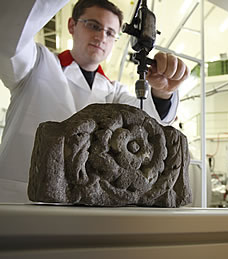
\includegraphics[width=.8\textwidth]{img/drill.jpg}
\caption{Entnahme der Probe, TRIGA Mainz.}
\end{figure}
\end{minipage}
\end{frame}

\begin{frame}{Schritt 2: Probenaufbereitung}
\begin{minipage}{0.5\textwidth}
\begin{figure}
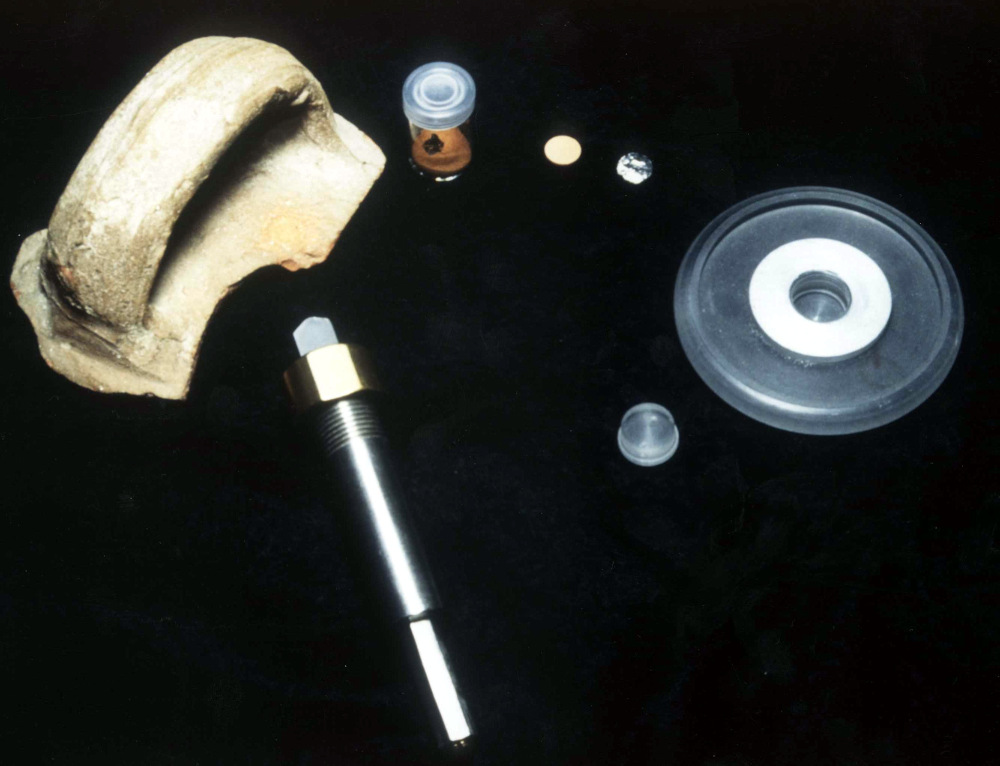
\includegraphics[width=\textwidth]{img/pill.jpg}
\caption{Objekt mit Bohrer, Tablette und Probenhalter, Mommsen 2002.}
\end{figure}
\end{minipage}\hfill
\begin{minipage}{.44\textwidth}\flushleft
\textbf{Bohrstaub wird zur Probe:}\smallskip

\begin{itemize}
\item chemisch reines Bindemittel, z.\,B.\ Zellulose
\item Herstellung einer \textbf{Tablette}
\item Durchmesser von 10\,mm und Dicke von 1\,mm
\item Feste Abmessungen wichtig für genaue Messung des $\gamma$-Spektrums!
\end{itemize}
\end{minipage}
\end{frame}

\subsection{Neutronenbestrahlung}

\begin{frame}{Schritt 3: Neutronenbestrahlung}
\begin{minipage}{0.52\textwidth}\flushleft
Als Neutronenquelle werden häufig \textbf{Kernreaktoren} benutzt.\smallskip

\begin{itemize}
\item Spaltung von Uranisotopen\\$\Rightarrow$ therm.\ Neutronen mit $0,025$\,eV
\item $10^{12}$ bis $10^{14}$ Neutronen pro Sekunde und cm$^2$
\item Ein Durchgang für mehrere Proben gleichzeitig
\item \alert{Referenztablette} mit bekannter Zusammensetzung
\end{itemize}
\end{minipage}\hfill
\begin{minipage}{0.44\textwidth}
\begin{figure}
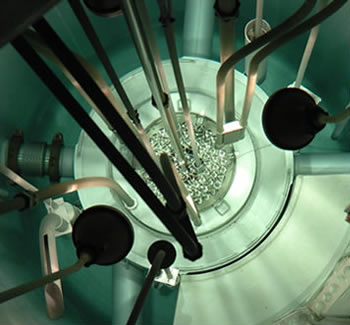
\includegraphics[width=\textwidth]{img/reactor-mainz.png}
\caption{TRIGA Reaktor, Mainz.}
\end{figure}
\end{minipage}
\end{frame}

\begin{frame}[<+->]{Einschub: Grundbegriffe Kernphysik}
\begin{enumerate}[(i)]
\item \textbf{Protonen} $p$ sind positiv geladene Teilchen mit Masse 1
\item \textbf{Neutronen} $n$ sind el.\ neutral geladene Teilchen mit Masse 1
\item Protonen und Neutronen fassen wir als \textbf{Nukleonen} zusammen
\item Protonenzahl (\textbf{Ordnungszahl}) $Z$ im Atomkern bestimmt das \emph{Element}
\item Nukleonenzahl (\textbf{Massenzahl}) $A$ im Atomkern bestimmt die \emph{Atommasse}
\item \textbf{Isotopen} sind Elemente mit unterschiedlicher Masse
\item Wir schreiben für Element X: \[\text{\ce{^A_Z X}\quad oder kurz \quad\ce{^A X}}\]
\end{enumerate}
\end{frame}

\begin{frame}{Neutronenaktivierung}
\begin{center}\vspace*{-2.5em}
\begin{tikzpicture}
\draw[color=white,line width=.01pt] (-7,-3) grid[xstep=7cm, ystep=3cm] (7,3);

\pgfbox[center,center]{\pgfuseimage{snucleus}};

\node at (-6.4,-1.1) {$n$};
\node at (-5.2,-3.5) {\Large \ce{^{A}_{Z} X}};
\node at (-2.3,-3.5) {\Large \ce{^{A+1}_{Z} X^*}};
\node at (.4,-3.5) {\Large \ce{^{A+1}_{Z} X}};
\node at (3.2,-3.5) {\Large \ce{^{A+1}_{Z±1} Y^*}};
\node at (6.1,-3.5) {\Large \ce{^{A+1}_{Z±1} Y}};
\node at (2.5,2) {\large $\beta^\pm$};
\node at (-0.7,-1.6) {\Large $\gamma$};
\node at (4.9,-1.6) {\Large $\gamma$};
\end{tikzpicture}
\end{center}
\end{frame}

\begin{frame}{Neutronenaktivierung: Beispiel}
\begin{figure}
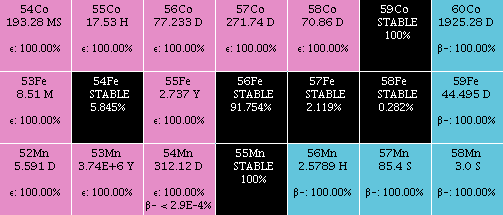
\includegraphics[height=.45\textheight]{img/nuclidchart.png}
\caption{Ausschnitt der Nuklidkarte.}
\end{figure}
\[\large\text{\ce{^{58} Fe \:(n,$\gamma$)\: ^{59}Fe ->[$\beta^-$][$T_{1/2}=45d$] ^{59} Co^* ->[][sofort] ^{59} Co + $\gamma$}}\]
\end{frame}

\begin{frame}{Schritt 4: $\gamma$-Spektroskopie}
\begin{minipage}{0.4\textwidth}\flushleft
\textbf{Messung der $\gamma$-Aktivität der Probe} zum Zeitpunkt $t$.\medskip

Messergebnis \alert{stark abhängig von $t$} wegen unterschiedlichen Halbwertszeiten, deswegen \textbf{mehrfach gemessen}!
\end{minipage}\hfill
\begin{minipage}{0.56\textwidth}
\begin{figure}
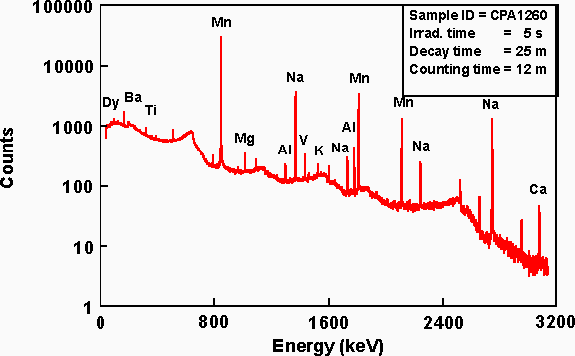
\includegraphics[width=\textwidth]{img/spect-1.png}
\caption{$\gamma$-Spektrum kurzlebiger El.\ einer Keramik-Probe, MURR.}
\end{figure}
\end{minipage}
\end{frame}

\begin{frame}{Schritt 4: $\gamma$-Spektroskopie}
\begin{figure}
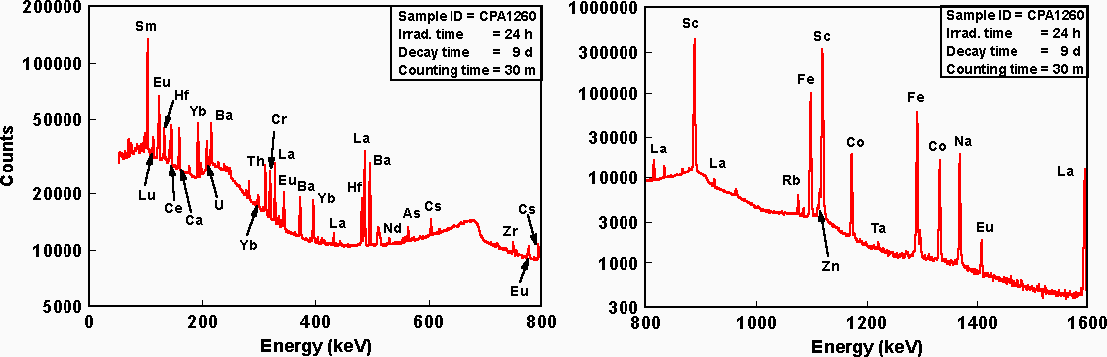
\includegraphics[width=\textwidth]{img/spect-2.png}
\caption{$\gamma$-Spektrum mittel- u.\ langlebiger El.\ einer Keramik-Probe, MURR.}
\end{figure}
\end{frame}

\subsection{Datenauswertung}

\begin{frame}{Schritt 5: Datenauswertung und Konzentrationsbestimmung}
\textbf{Wir haben gesehen:} Linien $\mapsto$ Elemente.
\begin{itemize}
\item 15--20 Linien aus Spektrum interessant
\item Mehrfachmessung einer Linie zu unterschiedlichen Zeiten
\item Korrekturen, z.\,B.\ bei Interferenzen und Überlappungen
\end{itemize}\medskip\pause

\textbf{Konzentrationsbestimmung:} Vergleich mit Referenzprobe!
\begin{itemize}
\item Jeweils Betrachtung eines Elements \textbf{in Probe und Referenz}:

\begin{center}
\alert{Intensitätsverhältnis $=$ Konzentrationsverhältnis}
\end{center}

(z.\,B.: Doppelte Linienstärke entspr.\ doppelter Konzentration)
\end{itemize}
\end{frame}

\begin{frame}{Schritt 5: Datenauswertung und Konzentrationsbestimmung}
\vspace*{-1em}
\Large Als Ergebnis erhalten wir den
\begin{huge}
\begin{center}
chemischen Fingerabdruck
\end{center}
\end{huge}
unserer Probe.
\end{frame}

\begin{frame}{Schritt 6: Mustervergleich}
\textbf{Gruppenbildung (\textit{Clustering)}:}
\begin{itemize}
\item Jede Probe $s$ ist ein \alert{Punkt} in einem $n$-dimensionalen Raum: \[s=(c_1,c_2,\dots,c_n)\] wobei $c_i$ die Konzentration des $i$-ten Elements in der Probe ist.
\item Ähnlich zusammengesetzte Proben liegen in einer \alert{Punktwolke}.
\item Finden von Punktwolken durch statistische Verfahren am Computer

\textbf{$\Rightarrow$ äquivalent zum Gruppieren der Proben!}
\end{itemize}
\end{frame}

\begin{frame}{Schritt 6: Mustervergleich}
\begin{minipage}{0.46\textwidth}\flushleft
Die Hyperräume werden durch \textbf{Diskriminanzanalyse} auf eine zweidimensionale Fläche projiziert.\medskip	

Z.\,B.\ 3 Gruppen: Mittelpunkte der Wolken spannen Projektionsebene auf.\bigskip

\begin{figure}
\caption{Beispiel für Gruppierungen nach Diskriminanzanalyse.}
\end{figure}
\end{minipage}\hfill
\begin{minipage}{0.5\textwidth}
\begin{figure}
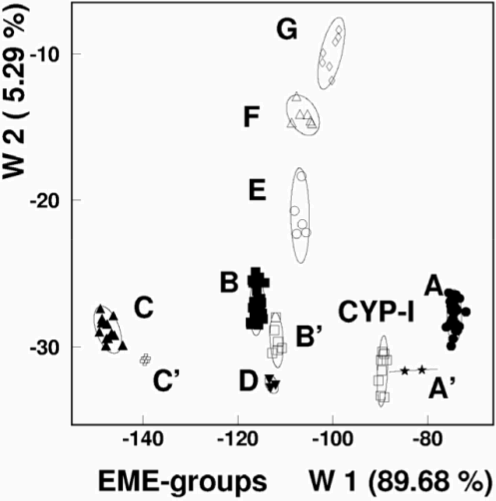
\includegraphics[width=.8\textwidth]{img/groups.png}
\end{figure}
\end{minipage}
\end{frame}

\section{Anwendungsbeispiel}

\section{Einrichtungen}

\section{Fazit}
\begin{frame}{Literatur}
\nocite{*}

\printbibliography[heading=none]
\end{frame}

\maketitle

\end{document}